\chapter{Metodi numerici}
Nei due capitoli precedenti abbiamo analizzato i fenomeni che regolano l'evoluzione dei dischi circum-stellari.
Per studiare il troncamento in dipendenza dei parametri della binaria, vogliamo ora risolvere numericamente le equazioni differenziali che descrivono il fenomeno in analisi. 
I metodi che vengono utilizzati per effettuare simulazioni idrodinamiche possono essere suddivisi in due macro-categorie:
\begin{list}{\textbf{-}}{\setlength{\itemsep}{0cm}}
    \item Euleriani
    \item Lagrangiani
\end{list}
Il criterio di suddivisione è il formalismo con cui vengono trattati i fluidi.
Il primo dei due approcci consiste nel descrivere il materiale per mezzo di grandezze che dipendono dalle coordinate spaziali e dal tempo, come per esempio: $\rho\left(\Vec{\textbf{x}},\,t\right)$ ed $u\left(\Vec{\textbf{x}},\,t\right)$.
I campi che sono soluzioni del problema idrodinamico nel caso euleriano consentono una descrizione del fluido in un sistema di riferimento che in generale non coincide con quello del fluido. Fissata una posizione $\Vec{\textbf{x}}_\textbf{p}$ nello spazio, il valore che assume una generica proprietà del fluido $a\left(\Vec{\textbf{x}}_\textbf{p}, t\right)$ varia al passare del tempo perché le condizioni nell'intorno di $\Vec{\textbf{x}}_\textbf{p}$ ne determinano un cambiamento locale. 
Il secondo approccio focalizza invece l'attenzione sulle proprietà del singolo elemento di fluido. Il punto di vista utilizzato è quello del materiale stesso, che viene considerato come costituito da un insieme di particelle lagrangiane: le proprietà del flusso sono funzione del particolare elemento.

\section{Mesh codes}

I metodi numerici che impiegheremo in questa tesi adottano il punto di vista euleriano: la regione simulata viene suddivisa mediante una griglia effettuando il passaggio dal continuo al discreto.

Studiamo per il momento un problema monodimensionale dove indichiamo con $x$ la posizione. Il dominio spaziale viene diviso in $n$ intervalli della stessa dimensione: una funzione $f(x,\,t)$ a tempo $t$ fissato assumerà n valori, in corrispondenza delle posizioni presenti nella griglia.
Per  valutare l'evoluzione della funzione nel tempo è necessario lavorare con intervalli $\Delta t$ finiti. I time-step non possono essere grandi a piacimento, ma devono rispettare la condizione CFL che pone un limite superiore a $\Delta t$ (vedi Sottosezione \ref{subsec:cond_CFL}).

La discretizzazione nel tempo e nello spazio del problema in analisi comporta che
\begin{equation}
x \in \textbf{\textit{R}} \qquad \qquad \rightarrow \qquad \qquad x \in \{x_1,\,x_2,\,\dots,\,x_n\},
\label{eq:discr_x}
\end{equation}
\begin{equation}
t \in \textbf{\textit{R}} \qquad \qquad \rightarrow \qquad \qquad t \in \{t^1,\,t^2,\,\dots,\,t^m\},
\label{eq:discr_t}
\end{equation}
\begin{equation}
f(x,\,t) \qquad \rightarrow \qquad \{f_1^1,\,f_2^1\,\dots\,f_n^1\}\,\dots\,\{f_1^m,\,f_2^m\,\dots\,f_n^m\},
\label{eq:discr_f}
\end{equation}
dove abbiamo indicato con $x_i$ il centro della i-esima cella.
Nella \eqref{eq:discr_f} l'indice a pedice indica la posizione in cui è stata valutata $f(x,\,t)$, mentre l'apice indica il tempo a cui è stata effettuata la stima.

\subsection{Metodo alle differenze finite} \label{subsec:diff_fin}

Il metodo alle differenze finite è una tecnica numerica di risoluzione di equazioni differenziali che si basa sull'approssimazione delle derivate di $f(x,\,t)$.
Vogliamo discretizzare la derivata fatta rispetto alla coordinata spaziale: per ottenere questo risultato sfruttiamo il fatto che $\partial f/\partial x$ è definita come il limite del rapporto incrementale in $x$.
Dato che la coordinata spaziale $x \in \{x_1,\,x_2\,\dots\,x_n\}$, possiamo approssimare la derivata di $f(x,\,t)$ sul bordo di una cella come
\begin{equation}
\frac{\partial f}{\partial x}\bigg|_{i+1/2}^j\,=\,\frac{f_{i+1}^j\,-\,f_{i}^j}{x_{i+1}\,-\,x_{i}}.
\label{eq:der_discr_x_limc}
\end{equation}
Assumiamo che la derivata ottenuta con il metodo delle differenze finite è la miglior stima di $\partial f/\partial x$ nel punto medio fra quelli utilizzati per calcolarla: l'indice $1/2$ nella \eqref{eq:der_discr_x_limc} indica che la derivata è valutata sulla superficie di separazione fra due celle adiacenti.
La derivata può essere determinata nel centro di una cella considerando i valori che $f(x,\,t)$ assume nelle due adiacenti:
\begin{equation}
\frac{\partial f}{\partial x}\bigg|_{i}^j\,=\,\frac{f_{i+1}^j\,-\,f_{i-1}^j}{x_{i+1}\,-\,x_{i-1}}.
\label{eq:der_discr_x_cenc}
\end{equation}
La discretizzazione del problema comporta l'insorgere di errori di troncamento: per determinarne l'entità lavoriamo con delle opportune espansioni di Taylor per una generica funzione $g(x)$. 

La 'forward derivative' è accurata al primo ordine: in questo caso la derivata è valutata ad uno dei due estremi utilizzati per calcolarla.
Considerando l'espansione di Taylor per $g(x+\Delta x)$ opportunamente riorganizzata
\begin{equation}
\frac{\partial g}{\partial x}\bigg|_{x}\,=\,\frac{g(x+\Delta x)\,-\,g(x,\,t)}{\Delta x}\,+\,O(\Delta x),
\label{eq:forward_der}
\end{equation}
osserviamo come l'errore di troncamento sia $O(\Delta x)$.

Lavoriamo ora con le espansioni per $g(x+\Delta x)$ e $g(x-\Delta x)$ arrestate al secondo ordine:
\begin{equation}
g(x+\Delta x)\,=\,g(x)\,+\,g'(x)\Delta x\,+\,O(\Delta x ^ 2),
\label{eq:espt_1}
\end{equation}
\begin{equation}
g(x-\Delta x)\,=\,g(x)\,-\,g'(x)\Delta x\,+\,O(\Delta x ^ 2),
\label{eq:espt_2}
\end{equation}
dove $'$ indica una derivazione rispetto alla variabile $x$.
Effettuando la differenza fra le due otteniamo 
\begin{equation}
g'(x)\,=\,\frac{g(x+\Delta x)\,-\,g(x-\Delta x)}{2\Delta x}\,+\,O(\Delta x^2)
\label{eq:centr_der}
\end{equation}
La \eqref{eq:centr_der} è valutata nel punto medio fra i due utilizzati per calcolarla: è detta derivata centrale ed è accurata al secondo ordine. Un analogo ragionamento può essere applicato alla derivata rispetto alla coordinata temporale.\\

L'algoritmo di Verlet è un tipico esempio di metodo alle differenze finite. Supponiamo di avere un sistema con configurazione $\Vec{r}(t)$ e di volerne determinare l'evoluzione al tempo $t\,+\,\delta t$. Proseguiamo come in precedenza considerando le seguenti espansioni di Taylor:
\begin{equation}
\Vec{r}(t\,+\,\delta t)\,=\,\Vec{r}(t)\,+\,\Vec{v}(t)\delta t\,+\,\frac{1}{2}\Vec{a}(t)\delta t^2\,+\,\frac{1}{6}\dot{\Vec{a}}(t)\delta t^3\,+\,O(\delta t^4),
\label{eq:exp1_verlet}
\end{equation}
\begin{equation}
\Vec{r}(t\,-\,\delta t)\,=\,\Vec{r}(t)\,-\,\Vec{v}(t)\delta t\,+\,\frac{1}{2}\Vec{a}(t)\delta t^2\,-\,\frac{1}{6}\dot{\Vec{a}}(t)\delta t^3\,+\,O(\delta t^4),
\label{eq:exp2_verlet}
\end{equation}
Sottraendo membro a membro le due equazioni ricaviamo che
\begin{equation}
\Vec{r}(t\,+\,\delta t) \simeq 2 \Vec{r}(t)\,-\,\Vec{r}(t\,-\,\delta t)\,+\,\Vec{a}(t)\delta t^2\,+\,O(\delta t^4).
\label{eq:pos_succ}
\end{equation}
L'errore di troncamento dell'algoritmo presentato è $O(\delta t^4)$: l'elevata precisione è dovuta all'utilizzo sia della configurazione al tempo $t$ che quella al tempo $t\,-\,\delta t$ per la determinazione della posizione successiva.
Oltre che per le ODE, il metodo può essere utilizzato per le PDE poiché il campo è noto in tutto il dominio simulato. 
Per una \textit{partial differential equation} il valore della posizione al tempo $t\,+\,\delta t$ non viene infatti determinato mediante la sola dipendenza temporale, ma anche in base ai valori del campo nell'intorno del sito considerato al tempo $t$.

\subsection{Condizione CFL} \label{subsec:cond_CFL}

La condizione di Courant-Friedrichs-Lewy fornisce un limite superiore all'intervallo temporale che può essere utilizzato per effettuare l'evoluzione del sistema: tale restrizione è necessaria per avere la convergenza delle soluzioni alle equazioni differenziali.
Il $\Delta t$ deve rispettare la condizione
\begin{equation}
\Delta t\,<\,C\,\frac{\Delta x}{u},
\label{eq:cond_deltaT}
\end{equation}
dove $C$ è un numero reale detto \textit{numero di Courant} e $\Delta x$ è l'estensione spaziale della singola cella. 
La condizione che abbiamo appena introdotto è evidentemente locale, dato che la velocità del fluido solitamente varia nel dominio considerato. Per ottenere il corretto intervallo che garantisca la convergenza della soluzione si valuta $\Delta t$ per ogni cella, per poi scegliere come fattore limitante il minore di tutti.

\section{Fargo3D}

FARGO3D è un codice magneto-idrodinamico sviluppato con l'obiettivo di studiare la fisica dei dischi proto-planetari e le loro interazioni con pianeti in formazione. Le equazioni differenziali caratteristiche del problema (vedi Sezione \ref{sec:mod_disc}) sono risolte utilizzando una griglia euleriana, che può essere applicata a sistemi di coordinate cartesiani, cilindrici o sferici. Le tecniche numeriche di risoluzione utilizzate sono il metodo alle differenze finite (esposto nella Sottosezione \ref{subsec:diff_fin}) ed il metodo ai volumi finiti.

\subsection{FARGO algorithm} \label{subsec:Fargo_al}

Per risolvere le equazioni idrodinamiche ed aggiornare il sistema FARGO3D utilizza un metodo time-explicit, implementando tecniche di 'operator splitting' ed 'upwind' \parencite{Fargo3D}: l'algoritmo utilizzato è iterativo e consente di calcolare esplicitamente le quantità al tempo $t\,+\,\Delta t$ in dipendenza del loro valore al tempo $t$.

Le equazioni differenziali idrodinamiche si presentano come equazioni di conservazione
\begin{equation}
\frac{\partial Q}{\partial t}\,+\,\nabla \cdot (Q\mathbf{v})\,=\,S(Q,\,\mathbf{v},\,t),
\label{eq:idr_tipo}
\end{equation}
dove $Q$ può essere una qualsiasi quantità ed $S$ indica le sorgenti o i pozzi di $Q$.
La tecnica di 'operator splitting' consiste nella separazione della \eqref{eq:idr_tipo} in due parti ciascuna delle quali viene risolta in uno step ad essa dedicata:
\begin{list}{\textbf{-}}{\setlength{\itemsep}{0cm}}
    \item il \textit{source step}, efettuato con tecniche alle differenze finite
    \item il \textit{transport step}, gestito con metodi numerici a volumi finiti
\end{list}
La variabile $Q_0\,=\,Q(t_0)$ viene aggiornata a $Q_1$ durante il 'source step', descritto da
\begin{equation}
\frac{\partial Q}{\partial t}\,=\,S(Q,\,\mathbf{v},\,t).
\label{eq:source_step}
\end{equation}
Il valore $Q_2\,=\,Q(t_0+\Delta t)$ viene ottenuto partendo da $Q_1$ mediante il 'transport step', che è strutturato come:
\begin{equation}
\frac{\partial Q}{\partial t}\,+\,\nabla \cdot (Q\mathbf{v})\,=\,0.
\label{eq:transport_step}
\end{equation}

In Figura \ref{fig:update_far} è riportato il processo di update delle varie quantità caratteristiche del fluido: dato che il codice è stato sviluppato per trattare problemi di magneto-idrodinamica sono presenti dei sub-step riguardanti la gestione dei fenomeni magnetici.
Il sesto substep è fondamentale per quanto riguarda la convergenza delle soluzioni perché viene imposta la 'CFL condition'.
L'intervallo $\Delta t$ selezionato ha una dipendenza sulla risoluzione della griglia: più piccole sono le celle utilizzate, più stringente sarà la condizione sul time step.
Inoltre il materiale costituente il disco orbita con velocità azimutali maggiori più vicino si trova alla stella: utilizzare $r_{min}$ troppo piccoli potrebbe risultare computazionalmente pesante, poiché la velocità $u$ a denominatore della \eqref{eq:cond_deltaT} potrebbe risultare troppo elevata.
I dischi d'accrescimento con aspect-ratio minore di uno sono caratterizzati da una dinamica super-sonica come evidenziato nella Sottosezione \ref{subsec:str_vert_disc}: dato che $v_{\varphi} \gg c_s$ la condizione CFL renderebbe inefficiente la simulazione.

FARGO3D, acronimo di \textit{Fast Advection in Rotating Gaseous Objects 3D}, è stato sviluppato con l'obiettivo di migliorare le performance del \textit{trasport step} per trattare oggetti in rapida rotazione.

L'idea alla base delle 'orbital advection techniques' è di decomporre per ogni anello di celle a raggio e colatitudine fissati la velocità azimutale $v$ in due componenti:
\begin{list}{\textbf{-}}{\setlength{\itemsep}{0cm}}
    \item $v^0$, che è una velocità uniforme in tutto l'anello considerato
    \item $\delta v$, che è una velocità residua (più piccola di $v^0$)
\end{list}
Questo modo di procedere consente di trattare ogni singolo anello dal punto di vista di un sistema quasi co-rotante con l'anello stesso: nella condizione di Courant verranno allora considerate solo le velocità $\delta v$ e $v_r$, consentendo l'utilizzo di $\Delta t$ maggiori.

\subsection{Griglia e campi} \label{subsec:MeshField}

La griglia è formata da $n_x$ celle in X, $n_y\,+\,2\cdot n_{ghy}$ celle in Y ed $n_z\,+\,2\cdot n_{ghz}$ celle in Z. I termini $ n_{ghy}$ ed  $n_{ghz}$ indicano il numero di 'ghost cells' poste accanto alla regione effettivamente simulata: queste celle sono fondamentali per l'implementazione delle 
\begin{figure}[H]
    \centering
    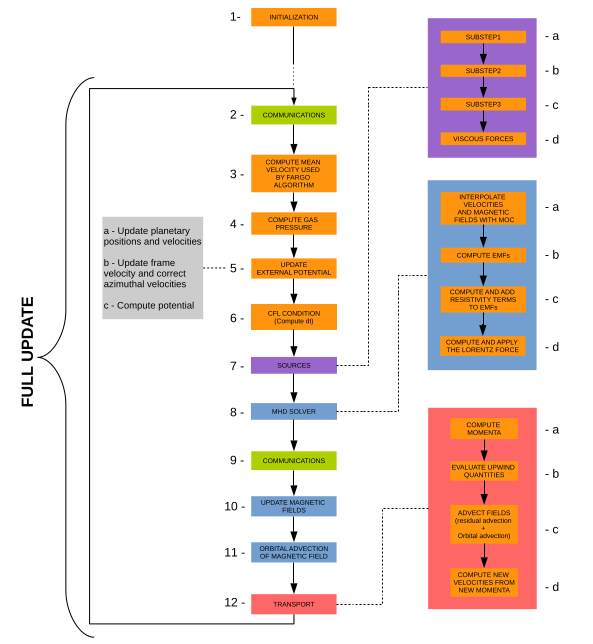
\includegraphics[width=\textwidth]{Immagini/Simulazioni/Update_FARGO.png}
    \caption{Schema riassuntivo delle operazioni performate in successione durante un update del sistema. Le parti con sfondo blu riguardano il caso di simulazioni magneto-idrodinamiche MHD \parencite{Fargo3D}.}
    \label{fig:update_far}
\end{figure}
condizioni al contorno.
Quando il codice viene eseguito in parallelo la griglia viene divisa in sotto-griglie in modo tale che ogni processore ne gestisca una: la regione simulata è sezionate in modo tale da rendere il più efficiente possibile l'esecuzione del programma.
La griglia può essere creata con coordinate cartesiane, cilindriche o sferiche:
\begin{table}[H]
\begin{center}
\begin{tabular}{|C{2cm}|C{2.5cm}|C{2.5cm}|C{2.5cm}|}
\hline
\rowcolor{yellow}
Coordinate & Variabile X & Variabile Y & Variabile Z\\
\hline
Cartesiane & x & y & z \\
\hline
Cilindriche & azimuth & raggio & z  \\
\hline
Sferiche & azimuth & raggio & colatitudine \\
\hline
\end{tabular}
\caption{Corrispondenza fra nome delle variabili e coordinate nelle varie geometrie \parencite{Fargo3D}.}
\label{tab:coor_Fargo3D}
\end{center}
\end{table}
I campi sono delle strutture di dimensione analoga a quella della griglia e consentono di memorizzare le variabili di interesse per la simulazione. 
I campi si dividono in due categorie:
\begin{list}{\textbf{-}}{\setlength{\itemsep}{0cm}}
    \item centrati, ossia che assumono valore al centro della cella
    \item sfalsati, ossia che contengono variabili definite sulle frontiere delle singole cellette.
\end{list}
Una cella di una tipica griglia di FARGO3D si presenta come in Figura \ref{fig:campi_far}.

\begin{figure}[h]
    \centering
    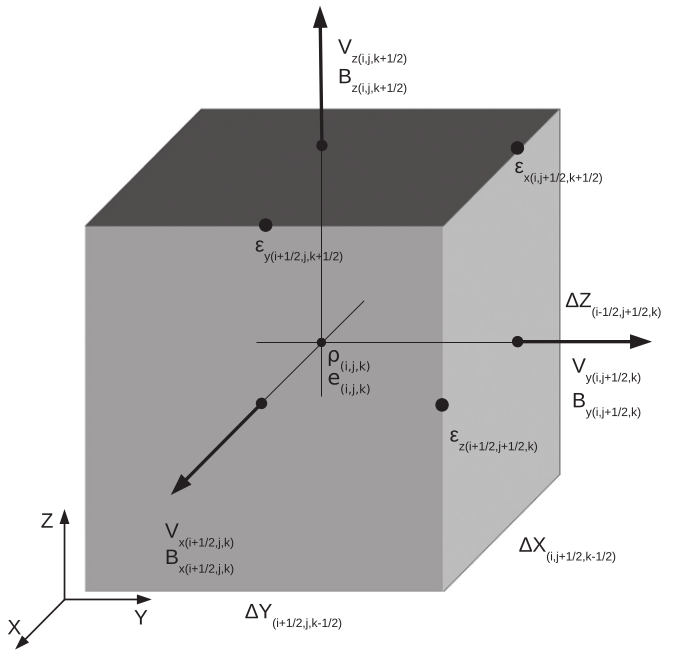
\includegraphics[width=0.8\textwidth]{Immagini/Simulazioni/CellaTipoFargo3D.png}
    \caption{Esempio di una cella in FARGO3D: le quantità vettoriali come la velocità sono poste sulle facce, mentre le quantità scalari come la densità sono poste al centro della cella \parencite{Fargo3D}.}
    \label{fig:campi_far}
\end{figure}

\subsection{Condizioni al contorno} \label{subsec:con_cont_far}

Le condizioni al contorno possono essere selezionate solo per le direzioni Y e Z. La direzione X è sempre considerata periodica perché FARGO3D è stato sviluppato per studiare i dischi d'accrescimento: lavorando in coordinate cilindriche X è l'azimuth e la richiesta di periodicità è necessaria per la definizione del setup.
La griglia, oltre alle celle attive, presenta anche delle celle fantasma che non fanno parte della regione simulata: queste 'ghost cells' vengono utilizzate per imporre le condizioni al contorno.
Le 'boundary condition BC' riguardano tutti i campi fondamentali e possono influenzare fortemente la dinamica del sistema simulato.
Le condizioni al contorno standard sono:
\begin{list}{\textbf{-}}{\setlength{\itemsep}{0cm}}
    \item \textit{Symmetric}, in cui il valore contenuto nella cella reale è copiato in quella fantasma. Tale BC è implementata sia per campi centrali che per campi sfalsati
    \item \textit{Antisymmetric}, che è implementata solo per i campi sfalsati. Questa BC determina una riflessione, poiché nella ghost-cell viene memorizzato l'opposto di quanto presente nella cella attiva
    \item \textit{Noboundary}, che consiste in una casistica senza BC.
\end{list}
Sono implementate anche delle condizioni al contorno specificatamente per il caso di disco kepleriano bidimensionale. Queste BC sono:
\begin{list}{\textbf{-}}{\setlength{\itemsep}{0cm}}
    \item \textit{Keplerian2Ddens}, che consiste in un'estensione analitica del profilo di densità alle celle adiacenti la griglia simulativa.
    \item \textit{Keplerian2Dvazim}, che consente di estrapolare il profilo di velocità Kepleriano
\end{list}
Un'ulteriore condizione al contorno è \textit{open}, implementata per la velocità radiale $v_r$ ai limiti della griglia: il materiale può uscire dalla regione simulata, ma non entrarvi.\\
\newpage
\textbf{Damping}\\

In FARGO3D è possibile specializzare delle zone della griglia in modo tale che si oppongano alla formazione di onde e perturbazioni di densità.
Le regioni in cui viene applicato il damping sono adiacenti alle frontiere: due parametri consentono di aumentarne oppure ridurne le dimensioni.
Lo smorzamento avviene con un tempo caratteristico $\tau_D$: più alto sarà il suo valore, minore sarà l'effetto totale.

Il damping agisce sulla densità e sulle velocità per imporre nuovamente le condizioni iniziali. 
Lo smorzamento non avviene ovunque con la stessa intensità, ma è massimo ad $r_{min}$ ed $r_{max}$, per poi diminuire con continuità fino agli altri limiti delle dumping zones.\\

\subsection{N-body solver}

In FARGO3D è possibile includere nella simulazione (non necessariamente nel dominio simulato) delle masse puntiformi che possono interagire sia fra sé stesse che con il gas.
\'E necessario specificare la distanza $d$ del pianeta dall'origine del sistema di riferimento e la sua massa: nel caso di orbita eccentrica $d$ corrisponde al semiasse maggiore. 

I pianeti sono inizializzati al tempo $t\,=\,0$ tutti con la stessa eccentricità e nella posizione che corrisponde al loro apoastro.

\subsection{Viscosità ed equazione di stato}

FARGO3D consente di lavorare con due moduli differenti per quanto riguarda la viscosità: \textit{Viscosity} ed \textit{Alphaviscosity}. 
Il primo dei due utilizza $\nu$ per riferirsi alla viscosità del materiale simulato, mentre il secondo consente di lavorare con $\alpha$ (vedi Sottosezione \ref{subsec: viscosity}).

Ulteriori specifiche per la definizione del setup riguardano l'equazione di stato. Anche in questo caso le possibili scelte sono due: \textit{Adiabatic} e \textit{Isothermal}.
Nel primo caso si utilizza l'equazione di stato \eqref{eq:eq_state}: il campo energia corrisponde all'energia interna per unità di volume $e$. Lavorando con \textit{Isothermal} l'equazione di stato assume invece la forma \eqref{eq:isothermal} ed il campo energia conterrà in realtà la velocità del suono nel fluido.

\subsection{Test idrodinamici: spreading ring}

In Figura \ref{fig:test_idro} è riportato uno dei test effettuati dagli sviluppatori di FARGO3D per verificare la validità del modello viscoso utilizzato. Tale verifica consiste nel risolvere numericamente il problema della diffusione di un anello gassoso (vedi sezione \ref{sec:spreading-ring}).
Al tempo $t\,=\,0$ il materiale si trova in un anello Kepleriano simmetrico rispetto a rotazioni attorno all'asse z: la viscosità cinematica utilizzata è $\nu\,=\,10^{-5}$. L'estensione radiale della griglia è $0.1\leq r \leq 1.6$: vengono usate 512 celle equamente spaziate. Il profilo di densità riportato in Figura \ref{fig:test_idro} presenta un buon accordo con l'espressione analitica confermando la solidità del codice FARGO3D.
\begin{figure}[H]
    \centering
    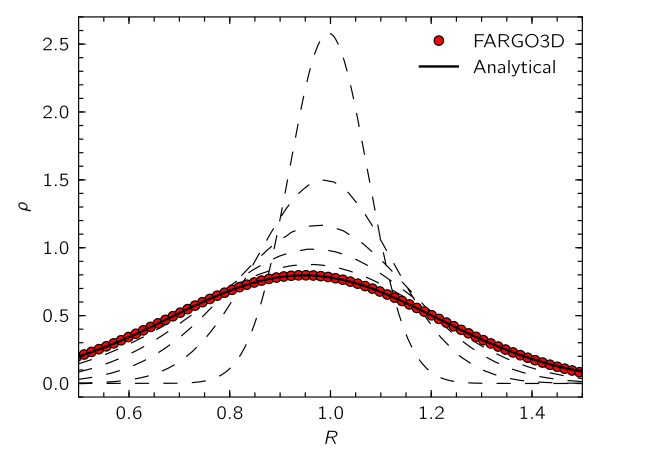
\includegraphics[height=9cm, width=10cm]{Immagini/Simulazioni/TestIdrodinamico.png}
    \caption{Test del modulo viscoso: evoluzione di un anello di materiale gassoso. Le linee tratteggiate corrispondono ai risultati numerici per tempi $t\,=\,100,\,300,\,500,\,700,\,900.$ La linea continua è la soluzione rappresenta la soluzione analitica a tempo $t\,=\,1100$, mentre i punti rossi sono i risultati numerici allo stesso istante di tempo \parencite{Fargo3D}.}
    \label{fig:test_idro}
\end{figure}


